\section*{Ejercicio 1}
\graphicspath{{Figuras/ej_01/}}

Comenzamos simulando la dinamica de dos neuronas Hogdkin-Huxley \cite{HH} conectadas simétricamente con interacciones sinapticas excitatorias e inhibitorias. Se utilizo una corriente externa $I_{\text{ext}}=10\,\text{mA}$ de manera que las neuronas estén oscilando periódicamente. La corriente de interacción sinaptica esta dada por
\begin{equation}
    I_{syn}(t) = -g_{syn} s(t) (V-V_{syn}),
\end{equation}
donde
\begin{align}
    \frac{ds}{dt}&= \frac{s_\infty(V) - s}{\tau}\\
    s_\infty(V)&= 0.5(1+\text{tanh}(\nicefrac{V}{5})),
\end{align}
siendo $V$ es el potencial de  la neurona y $\tau$ es el tiempo característico asociado a la inhibición, el cual se tomo como $\tau = 3\,\text{ms}$ durante todo el trabajo.

Se busco estudiar el desfasaje entre las neuronas y la tasa de disparo del sistema como función del parámetro $g_{syn}$ para valores entre $0$ y $2\,\frac{\text{mS}}{\text{cm}^2}$. Este estudio realizo tanto para interacciones excitatorias como inhibitorias, tomando $V_{syn}=0\,\text{mV}$ y $V_{syn}=-80\,\text{mV}$ respectivamente.


\begin{figure}[h!]
    \centering
    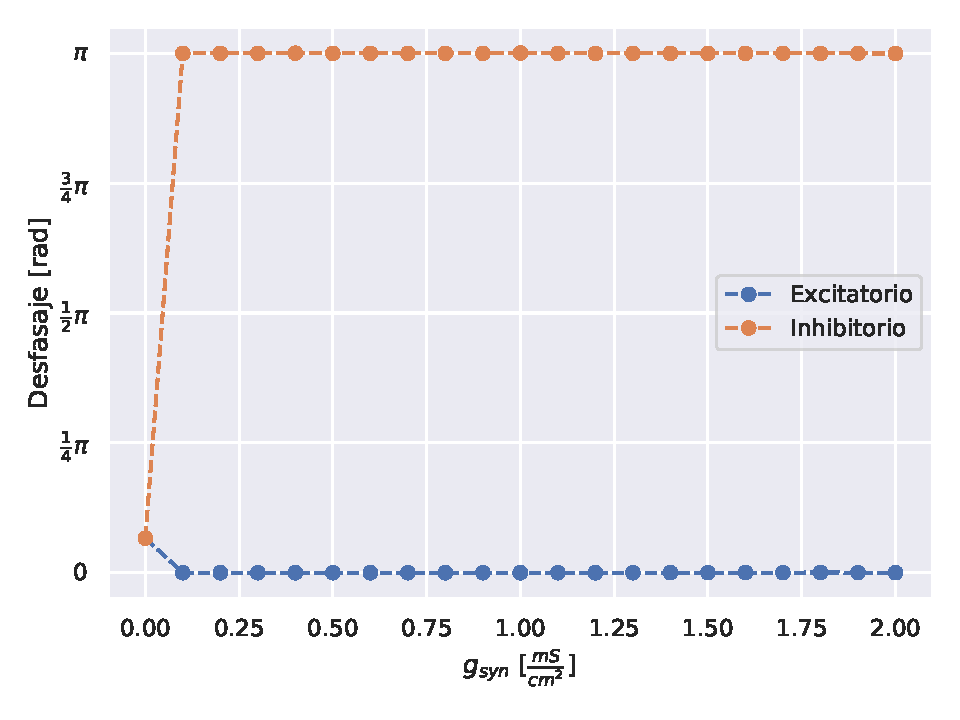
\includegraphics[width=0.6\textwidth]{Desfasaje.pdf}
    \caption{Caption.}
    \label{ej01:Desfasaje}
\end{figure}

\begin{figure}[h!]
    \centering
    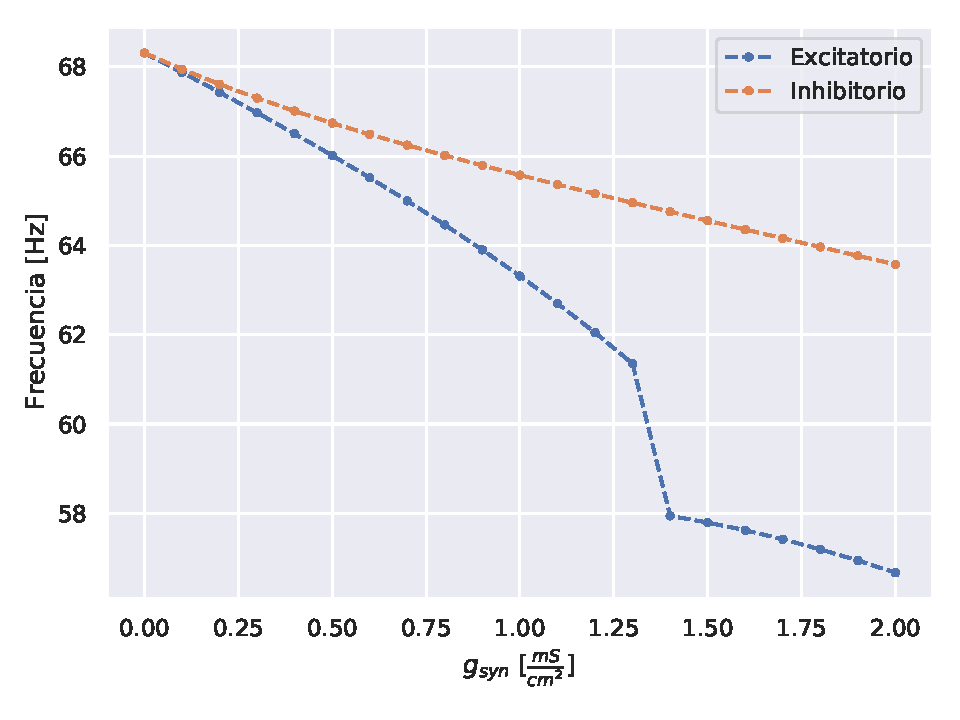
\includegraphics[width=0.6\textwidth]{Tasa_de_Disparo.pdf}
    \caption{Caption.}
    \label{ej01:tasaDeDisparo}
\end{figure}

En la Figura \ref{ej01:tasaDeDisparo} se observa la frecuencia del sistema acoplado como función del parámetro $g_{syn}$, el cual influye en la intensidad de la interacción. Se observa la disminución de la frecuencia de las neuronas con el aumento del valor de $g_{syn}$. Para la curva correspondiente a la interacción excitatoria, esta disminución se debe a que la corriente $g_{syn}$ disminuye la corriente total dentro de la neurona. Por otro lado, para la interaccion excitatoria, se observa que la disminucion de la frecuencia es menos pronunciada, ya que el potencial inhibitorio ralentiza la frecuencia de los spikes de las neuronas, desfasandolos.